\documentclass{article}
\usepackage[utf8]{inputenc}
\usepackage{graphicx}
\usepackage{bigints}
\usepackage[left=25mm,top=10mm,right=25mm,bottom=5mm]{geometry}
\usepackage{amsmath}
\usepackage{array}

\title{\Huge \textbf{AE 238 Assignment 3}}
\author{\Huge \textbf{Krishna Wadhwani - 160010031 }}
\date{January 2018}


\begin{document}

\maketitle


\noindent \title{\LARGE \textbf{Question 1}}
\bigbreak
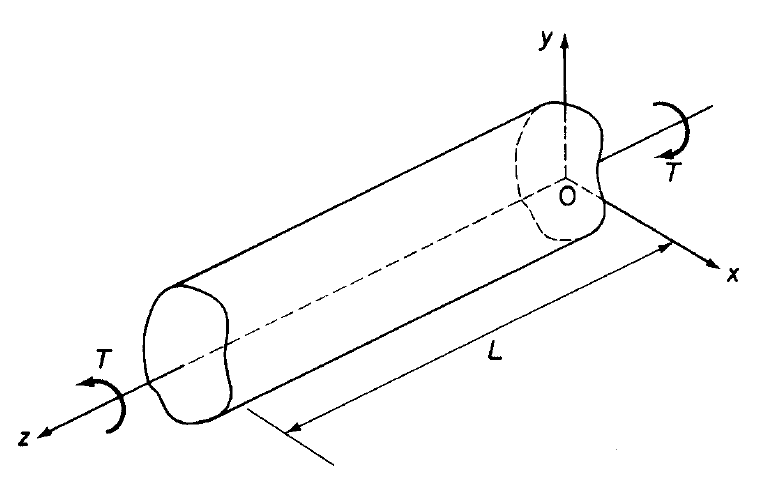
\includegraphics[scale=0.8]{1.png}\\
\noindent Our aim is to find the stress functions- prandtl ($\phi$) and St.Venants ($\psi$) and warping displacement for a cylindrical body with elliptical cross-section for different $\dfrac{a}{b}$ ratios. \\

\noindent My approach is that I will start by assuming paradtl stress fuction $\phi$ and the find a fucntion for the warping dispacement $w$ that satiisfies the St.Venant's stress function $\psi$\\

\noindent Since no direct loads are applied, we can safely assume $\sigma_{x}=\sigma_{y}=\sigma_{z}=0$ and that the torque resisted is solely due to shear stress in the plane of cross-section $\implies \tau_{xy}=0$\\

\noindent The stresses obtained from the stress function must satisfy the equations of equilibrium, compatibility and boundary conditions.  \\

\noindent \underline{Equilibrium equations}: \\

\noindent $\dfrac{\partial \tau_{xz}}{\partial z}=0$\\
$\dfrac{\partial \tau_{yz}}{\partial z}=0$\\
$\dfrac{\partial \tau_{xz}}{\partial x} + \dfrac{\partial \tau_{yz}}{\partial y}=0$\\

\noindent From the first two equations, we can infer that $\tau_{xz}$ is a function of $x$ and $\tau_{yz}$ is a function of $y$ which means that they are constant along the length of the bar which have same $x$ and $y$. 

\noindent From the 3rd equilibrium equation, we will assume $\phi$ such that equilibrium equations are trivially satisfied. Hence: we assume $\phi$ as: \\

\noindent $\dfrac{\partial \phi}{\partial x}= -\tau_{zy}$ \ \ \ $\dfrac{\partial \phi}{\partial y}= \tau_{zx}$\\

\noindent Note that $\phi$ is a function of $x$ and $y$ and hence trivially satisfies the equilibrium equation. \\

\noindent Now, from the assumed state of stress, we can also conclude that: \\
$\epsilon_x= \epsilon_y = \epsilon_z= \gamma_{xy}=0$\\
Also as $\tau_{zx}$ and $\tau_{zy}$ are functions of x and y respectively, so are the corresponding strains $\gamma_{zx}$ and $\gamma_{zy}$.\\

\noindent \underline{Compatibility equations}: \\

\noindent From the above strain criteria, the compatibility equation reduces to: \\

\noindent $\dfrac{\partial}{\partial x} \Big{(}-\dfrac{\partial \gamma_{zy}}{\partial x}+\dfrac{\partial \gamma_{zx}}{\partial y}\Big{)}=0$\\
$\dfrac{\partial}{\partial y} \Big{(}\dfrac{\partial \gamma_{zy}}{\partial x}-\dfrac{\partial \gamma_{zx}}{\partial y}\Big{)}=0$\\

\noindent $\implies \dfrac{\partial}{\partial x}\Big{(}\dfrac{\partial^2 \phi}{\partial x^2}+\dfrac{\partial^2 \phi}{\partial x^2} \Big{)}=0$\\

\noindent $\implies \dfrac{\partial}{\partial y}\Big{(}\dfrac{\partial^2 \phi}{\partial x^2}+\dfrac{\partial^2 \phi}{\partial x^2} \Big{)}$\\

\noindent Hence, gradient of $\Big{(}\dfrac{\partial^2 \phi}{\partial x^2}+\dfrac{\partial^2 \phi}{\partial x^2} \Big{)}$ is equal to 0: \\

\noindent $\implies \dfrac{\partial^2 \phi}{\partial x^2}+\dfrac{\partial^2 \phi}{\partial x^2}= F$ \\

where $F$ is a constant. \\

\noindent \underline{Boundary Condition}: \\

\noindent On the surface of the bar, there are no externally applied force and also, the direction cosine $n$ is 0, therefore $\overline{X}=\overline{Y}=\overline{Z}=0$. So we get: \\

\noindent $\tau_{yz}m+\tau_{xz}l=0$\\
As $l=\dfrac{dy}{ds}$ and $m=-\dfrac{dx}{ds}$ \\
$\implies \dfrac{\partial \phi}{\partial y}\dfrac{dy}{ds}+ \dfrac{\partial \phi}{\partial x}\dfrac{dx}{ds}  =0$\\
$\implies \dfrac{\partial \phi}{ds}= 0$\\
$\implies \phi=c$ \\

\noindent Hence, $\phi$ is constant on the surface of the bar. As this value of constant doesen't affect the value of stresses, we can conveniently take this value to be 0. \\

\noindent $\implies \phi=0$ on the surface\\

\noindent On the ends of the bar, $l=0, m=0, n=1$, so we get: \\
$\overline{X}=\tau_{zx}$\\ 
$\overline{Y}=\tau_{zy}$\\ 
$\overline{Z}=0$\\ 

\noindent Before assuming a $\phi$ for our give problem of elliptical cross-section, I will find the expression of sheer forces $S_x, S_y$, applied torque $T$ annd the warping displacement $w$ in terms of $\phi$. \\

\noindent \underline{Sheer forces}:\\

\noindent $S_x= \int \int \overline{X}dxdy= \int\int\tau_{zx}dxdy$\\
$\implies S_x= \bigint\bigint \dfrac{\partial\phi}{\partial y}dxdy$\\
$\implies S_x=\int dx\bigint\dfrac{\partial\phi}{\partial y}dx=0$ as $\phi=0$ at the boundary\\

\noindent Similarly $S_y=\int dy\bigint\dfrac{\partial\phi}{\partial x}dx=0$

\noindent Hence, there are no resultant forces on the ends of the bar and the forces represent a torque of magnitude $T$.\\
\newpage
\noindent \underline{Torque}:\\

\noindent $T=\int\Huge\int (\tau_{zy}x- \tau_{zx}y)dxdy$\\
$\implies T=-\bigint\bigint(\dfrac{\partial\phi}{\partial x}x + \dfrac{\partial\phi}{\partial y}y)dxdy$\\
Integrating by parts, we get:\\
$T=2\int\int\phi dxdy$ \\

\noindent \underline{Warping displacement}:\\

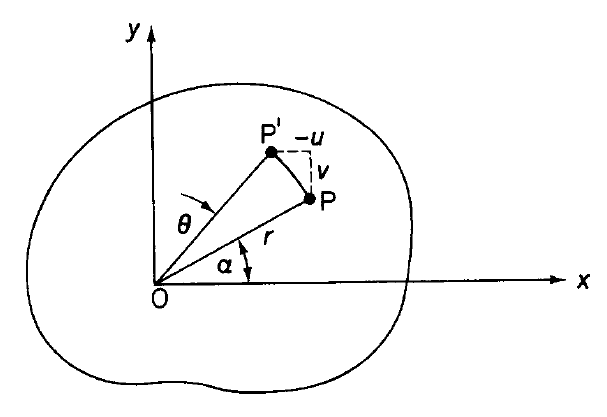
\includegraphics[scale=0.6]{2.png}\\

As $\epsilon_x=\epsilon_y=\epsilon_z=\gamma_{xy}=0$\\
$\implies \dfrac{\partial u}{\partial x}=\dfrac{\partial v}{\partial y}=\dfrac{\partial w}{\partial z}=\dfrac{\partial v}{\partial x}+\dfrac{\partial u}{\partial y}=0$\\

\noindent From this, we can infer that each cross-section rotates as a rigid body in its own plane about a centre of rotation or centre of twist. Although cross-sections suffer warping displacement $w$ normal to their planes, but the value of $w$ at points having same coordinates along the length of the bar are equal. Hence, each longitudinal fibre of the bar remains unrestrained. 

\noindent Let the cross-section of the bar rotate through a small angle $\theta$ about its centre of twist assumed coincident with the origin of the axes $O_{xy}.$ Let some point P$(r,\alpha)$ be dispaced to P$'(r, \alpha+\theta)$ (See the diagram above)\\

\noindent We have: \\

\noindent $u=-r\theta sin\alpha$, $v=r\theta cos\alpha$\\
$\implies u=-\theta y$, $v=\theta x$\\

\noindent Also we know that:\\

\noindent $\gamma_{xz}=\dfrac{\tau_{xz}}{G}=\dfrac{\partial u}{\partial z}+\dfrac{\partial w}{\partial x}$\\
$\gamma_{xy}=\dfrac{\tau_{zy}}{G}=\dfrac{\partial v}{\partial z}+\dfrac{\partial w}{\partial y}$\\

\noindent $\implies \dfrac{\partial w}{\partial x}= \dfrac{\tau_{zx}}{G}+ \dfrac{d\theta}{dz}x$\\
$\implies \dfrac{\partial w}{\partial y}= \dfrac{\tau_{zy}}{G}- \dfrac{d\theta}{dz}y$\\
Since each cross-section rotates as a rigid body, $\theta$ is a function of $z$ only.\\
As $\dfrac{\partial^2 w}{\partial y \partial x}=\dfrac{\partial^2 w}{\partial x \partial y}$\\
$\implies \dfrac{\partial^2 \phi}{\partial y^2}+\dfrac{\partial^2 \phi}{\partial x^2}=-2G\dfrac{d\theta}{dz}$\\

\noindent $-2G\dfrac{d\theta}{dz}=F$ from our earlier equation \\
\newpage

\noindent With these information, we will assume a suitable $\phi$ to solve the given problem. \\
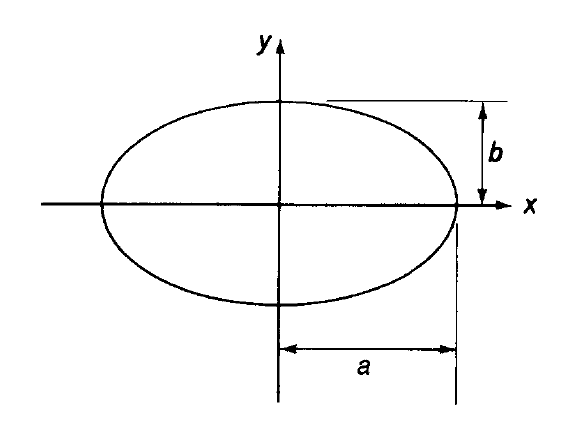
\includegraphics[scale=0.6]{4.png}\\
Let $\phi=A\Big{(}\dfrac{x^2}{a^2}+\dfrac{y^2}{b^2}-1\Big{)}$ \\

\noindent The assumed function satisfies the boundary condition as $\phi=0$ on the edge of the ellipse. 

\noindent From the compatibility equation: $\dfrac{\partial^2 \phi}{\partial x^2}+ \dfrac{\partial^2 \phi}{\partial y^2}=F$ \\
$\implies 2A\Big{(}\dfrac{1}{a^2}+\dfrac{1}{b^2}\Big{)}=F$\\

\noindent As we have earlier derived that $F=-2G\dfrac{d\theta}{dz}$\\
$\implies 2A(\dfrac{1}{a^2}+\dfrac{1}{b^2})=-2G\dfrac{d\theta}{dz} $\\
%$\implies A=-\dfrac{G\dfrac{d\theta}{dz}}{\dfrac{1}{a^2}+\dfrac{1}{b^2}}$\\
$\implies A=- \dfrac{Ga^2b^2}{a^2+b^2}\dfrac{d\theta}{dz}$ \\

\noindent So $\phi=- \dfrac{Ga^2b^2}{a^2+b^2}\dfrac{d\theta}{dz}\Big{(}\dfrac{x^2}{a^2}+\dfrac{y^2}{b^2}-1\Big{)}$\\

\noindent As we have derived earlier, $T=\int\int\phi dxdy$\\
$\implies T=- \bigint\bigint \dfrac{Ga^2b^2}{a^2+b^2}\dfrac{d\theta}{dz}\Big{(}\dfrac{x^2}{a^2}+\dfrac{y^2}{b^2}-1\Big{)}dxdy$\\
$\implies T=-\dfrac{Ga^2b^2}{a^2+b^2}\dfrac{d\theta}{dz}\bigint\bigint\Big{(}\dfrac{x^2}{a^2}+\dfrac{y^2}{b^2}-1\Big{)}dxdy$\\

\noindent Now, $\int\int x^2dxdy= I_{yy}$ and $\int\int y^2dxdy= I_{xx}$ \\

\noindent $\implies T=-\dfrac{Ga^2b^2}{a^2+b^2}\dfrac{d\theta}{dz}\Big{(}\dfrac{I_{yy}}{a^2}+\dfrac{I_{xx}}{b^2}- \pi ab\Big{)}$\\

\noindent For an ellipse, $I_{yy}=\dfrac{\pi a^3b}{4}$ and $I_{xx}= \dfrac{\pi ab^3}{4}$. Substituting these values, we get: \\

$\noindent T=G\dfrac{d\theta}{dz}\dfrac{\pi a^3b^3}{a^2+b^2} $\\

\noindent From torsion theory, $T=GJ\dfrac{d\theta}{dz}$\\
Hence for an ellipe, $J=\dfrac{\pi a^3b^3}{a^2+b^2}$\\

\noindent Hence stress function for our given problem: \\

$\mathbf{\phi=- \dfrac{T}{\pi ab} \Big{(}\dfrac{x^2}{a^2}+\dfrac{y^2}{b^2}-1\Big{)}}$\\

\noindent Expression for $\tau_{zx}$ and $\tau_{zy}$: \\

\noindent $\mathbf{\tau_{zx}=\dfrac{\partial\phi}{\partial y} =- \dfrac{2Ty}{\pi ab^3}}$\\

\noindent $\mathbf{\tau_{zy}=-\dfrac{\partial\phi}{\partial x} = \dfrac{2Tx}{\pi a^3b}}$\\

\noindent Expression for warping displacement: \\

\noindent We have derived that: \\
$\dfrac{\partial w}{\partial x}= \dfrac{\tau_{zx}}{G}+ \dfrac{d\theta}{dz}x$\\

\noindent Substituting the expression for $\tau_{zx}$ and $\dfrac{d\theta}{dz}$, we get:\\

\noindent $\dfrac{\partial w}{\partial x}=\dfrac{T}{G\pi a^3b^3}(b^2-a^2)y$\\
\noindent $\implies w=\dfrac{T}{G\pi a^3b^3}(b^2-a^2)xy+ f(y)$\\

\noindent Similarly for $\implies \dfrac{\partial w}{\partial y}= \dfrac{\tau_{zy}}{G}- \dfrac{d\theta}{dz}y$, we get:\\ 

\noindent $\mathbf{w=\dfrac{T}{G\pi a^3b^3}(b^2-a^2)xy+ g(x)}$ \\

\noindent As the warping dispacement given by both the equations must have same value at identical points $(x,y)$, $f(y)=g(x)=0$. Hence, the final expression for warping displacement is as follows \\

\noindent $w=\dfrac{T}{G\pi a^3b^3}(b^2-a^2)xy$\\

\noindent \underline{St. Venant function $\psi$}\\

\noindent By the definition of $\psi$:\\

\noindent $w=\psi \dfrac{d\theta}{dz}$\\
$\implies \psi=\dfrac{w}{d\theta/dz}$\\
$\implies \psi=\dfrac{T}{G\pi a^3b^3}(b^2-a^2)xy \times \dfrac{GJ}{T}$\\

\noindent $\implies \mathbf{\psi=xy\Big{(}\dfrac{b^2-a^2}{b^2+a^2}\Big{)}}$\\


\noindent \underline{Variation of $\tau_{zx}$ and $\tau_{zy}$}:\\

\begin{center}

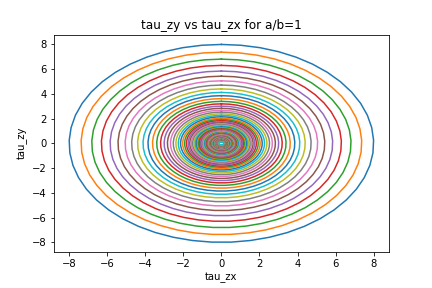
\includegraphics[scale=1]{AE238_A3_1.png}\\
\newpage
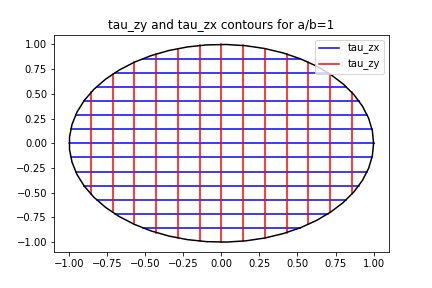
\includegraphics[scale=1]{AE238_A3_3.png}\\
\bigbreak
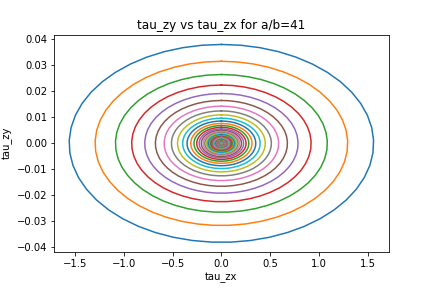
\includegraphics[scale=1]{AE238_A3_2.png}\\

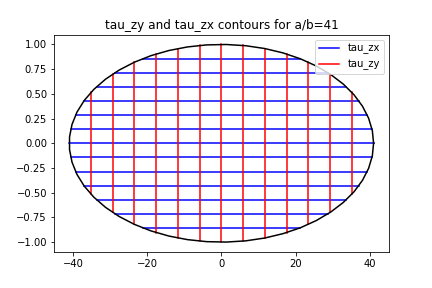
\includegraphics[scale=1]{AE238_A3_4.png}\\

\end{center}

\noindent Some important points about the graphs above:\\
\begin{itemize}
\item the graphs have been plotted in ipython notebook. 

\item In the above $\tau_{zy}$ vs $\tau_{zx}$ graphs, $\tau_{zy}$ is plotted in $y-$axis while $\tau_{zx}$ is plotted in x-axis. Notice the scale of $x$ and $y$ axes in both the cases. The resultant ellipse of the net shear stress gets smaller of increasing the $\dfrac{a}{b}$ ratio. \\
\item In $\tau_{zy}$ vs $\tau_{zx}$ graph for $\dfrac{a}{b}=1$, the contours are circular as evident by the values on $x$ and $y$ axes whereas for $\dfrac{a}{b}=41$, the contours are elliptical.  
\item In the above contour graphs, contours of $\tau_{zy}$ and $\tau_{zx}$ is shown within the elliptical cross-section. \\
\item Notice the scale of $x$ and $y$ axes in both the cases (explained in bullet point 1 and further in the last section of the assignment). The ellipse gets smaller of increasing the $\dfrac{a}{b}$ ratio. \\

\end{itemize}
\bigbreak
\noindent \underline{Location of maximum sheer stress}:\\

\noindent Let the resultant sheer stress be $\tau$.\\

$\tau=\sqrt{\tau_{zx}^2+\tau_{zy}^2}$\\
$\implies \tau= \dfrac{2T}{\pi ab}\sqrt{\dfrac{x^2}{a^4}+ \dfrac{y^2}{b^4}}$\\

\noindent \underline{For $a=b$}: \\
$\tau= \dfrac{2T}{\pi b^4}\sqrt{x^2+y^2}$\\

\noindent As $\dfrac{x^2}{a^2}+\dfrac{y^2}{b^2}\leq 1$ \\
$\dfrac{x^2}{b^2}+\dfrac{y^2}{b^2}\leq 1$\\
$x^2+y^2\leq b^2$\\

\noindent Hence: \\

\noindent $\tau_{max}= \dfrac{2T}{\pi b^3}$\\

\noindent Location of maximum sheer stress: circumference of the circle (same value at all points of the circumference)\\

\noindent \underline{For a general case: $a=rb$}: \\
$\tau= \dfrac{2T}{\pi rb^2}\sqrt{\dfrac{x^2}{r^4b^4}+ \dfrac{y^2}{b^4}}$\\
$\implies \tau= \dfrac{2T}{\pi rb^4}\sqrt{\dfrac{x^2}{r^4}+ y^2}$\\
\bigbreak
\noindent From the solution for $\dfrac{a}{b}=1$, it is intuitive that the shear stress will be maximum at the circumference of the ellipse and as we are solving for an ellipse, I am converting the above equation to polar coordinate. Hence, I am substituting:\\ $x=acos\theta$ $y=bsin\theta$\\

\noindent After this substitution: \\

\noindent $\tau= \dfrac{2T}{\pi rb^3}\sqrt{\dfrac{cos^2\theta}{r^2}+ sin^2\theta}$\\
$\implies \tau= \dfrac{2T}{\pi rb^3}\sqrt{1-\Big{(}1-\dfrac{1}{r^2}\Big{)}cos^2\theta} $

\noindent This value is maximized at $\theta=90^\circ$, i.e. , $x=0, y=b$. \\

\noindent $\tau_{max}=\dfrac{2T}{\pi rb^3}$\\

\noindent \underline{For $a=41b$}:\\

\noindent Substitute r=41 in the above expression for maximum shear stress: \\

\noindent $\tau_{max}=\dfrac{2T}{41\pi b^3}$\\

\noindent Location of maximum sheer stress: $x=0, y=b$\\








\end{document}
